%%%% Proceedings format for most of ACM conferences (with the exceptions listed below) and all ICPS volumes.
\documentclass[sigconf]{acmart}
%%%% As of March 2017, [siggraph] is no longer used. Please use sigconf (above) for SIGGRAPH conferences.

%%%% Proceedings format for SIGPLAN conferences 
% \documentclass[sigplan, anonymous, review]{acmart}

%%%% Proceedings format for SIGCHI conferences
% \documentclass[sigchi, review]{acmart}

%%%% To use the SIGCHI extended abstract template, please visit
% https://www.overleaf.com/read/zzzfqvkmrfzn


\usepackage{booktabs} % For formal tables
\usepackage{subfigure}
\usepackage{algorithmic}
\usepackage{amsthm}
% \usepackage{algorithm}
\usepackage[linesnumbered,ruled,vlined]{algorithm2e}
\usepackage{amsmath}
\usepackage{float}

% Copyright
%\setcopyright{none}
%\setcopyright{acmcopyright}
%\setcopyright{acmlicensed}
\setcopyright{rightsretained}
%\setcopyright{usgov}
%\setcopyright{usgovmixed}
%\setcopyright{cagov}
%\setcopyright{cagovmixed}


% DOI
% \acmDOI{10.475/123_4}

% ISBN
% \acmISBN{123-4567-24-567/08/06}

%Conference
\acmConference[FAT*ML19]{FAT* ML conference}{January 2019}{Atlanta, Georgia USA}
\acmYear{2019}
\copyrightyear{2018}


%\acmArticle{4}
%\acmPrice{15.00}

% These commands are optional
%\acmBooktitle{Transactions of the ACM Woodstock conference}
\editor{}
\editor{}
\editor{}


\begin{document}
\title{Pareto-Efficient Subgroup Fairness via the lens of Causality and Confounding Factors}
%\titlenote{Produces the permission block, and
%  copyright information}
% \subtitle{Extended Abstract}
%\subtitlenote{The full version of the author's guide is available as
%  \texttt{acmart.pdf} document}


% \author{Ananth Balashankar}
%\authornote{}
%\orcid{1234-5678-9012}
%\affiliation{%
%  \institution{New York University}
%  \streetaddress{}
%  \city{New York}
%  \state{NY}
%  \postcode{10003}
%}
%\email{ananth@nyu.edu}

%\author{Alyssa Lees}
%\authornote{}
%\affiliation{%
%  \institution{Google RMI NYC}
%  \streetaddress{}
%  \city{New York}
%  \state{NY}
%  \postcode{10012}
%}
%\email{AlyssaLees@google.com}


% The default list of authors is too long for headers.
% \renewcommand{\shortauthors}{A. Balashankar et al.}


\begin{abstract}
Recent literature aimed at resolving concerns of inequity in machine learning models is often predicated on defining constraints with respect to specific predefined sensitive variables.  A sensitive variable is a feature, such as race or gender in a dataset containing user info, that should not exhibit conditionally discriminative behavior in output classification. Ensuring subgroup fairness based on the intersectionality of multiple sensitive variables in a dataset is critical for bias mitigation algorithms. Scaling existing bias minimizing techniques, such as equalizing odds, to ensure subgroup fairness may lead to scenarios where hard equality constraints are impossible to achieve. Similarly, relaxation of these constraints may lead to degradation in performance. Explicitly we explore edge-case scenarios where regularization of these sensitive variables via Lagrangian relaxation can exacerbate classification inequity within subgroups.  \par
In order to mitigate, we propose a softer constraint based on Pareto-efficiency which leads to better subgroup performance.  We also jointly explore how detection of potential causal confounding variables can drastically change the interpretation of fairness after adjusting for sensitive variable bias.  In such situations, interventions by domain experts may be necessary to interpret the confounding variables and to offer a holistic understanding of the tradeoffs in subgroup fairness.  We propose a methodology to identify and incorporate possible confounding variables into sensitive variable analysis to aid in this pursuit.  Evaluation on synthetic data and the UCI Adult dataset highlights the utility and increased performance with our approach.

\end{abstract}

%
% The code below should be generated by the tool at
% http://dl.acm.org/ccs.cfm
% Please copy and paste the code instead of the example below.
%


\maketitle

% \section{Introduction}

The \textit{proceedings} are the records of a conference.\footnote{This
  is a footnote}  ACM seeks
to give these conference by-products a uniform, high-quality
appearance.  To do this, ACM has some rigid requirements for the
format of the proceedings documents: there is a specified format
(balanced double columns), a specified set of fonts (Arial or
Helvetica and Times Roman) in certain specified sizes, a specified
live area, centered on the page, specified size of margins, specified
column width and gutter size.
\subsection{Our Results and Contributions}
\subsection{Further Related Work}
Kilbertus et al, propose a way of identifying proxy variables based on correlation or prior knowledge in a causal graph and provides ways of intervening on these proxy variables and ensuring probability of outcome given all variations of proxy variables is the same in simple linear models.

\section{Models and Fairness Metric Preliminaries}
Typically, the body of a paper is organized into a hierarchical
structure, with numbered or unnumbered headings for sections,
subsections, sub-subsections, and even smaller sections.  The command
\texttt{{\char'134}section} that precedes this paragraph is part of
such a hierarchy.\footnote{This is a footnote.} \LaTeX\ handles the
numbering and placement of these headings for you, when you use the
appropriate heading commands around the titles of the headings.  If
you want a sub-subsection or smaller part to be unnumbered in your
output, simply append an asterisk to the command name.  Examples of
both numbered and unnumbered headings will appear throughout the
balance of this sample document.

Because the entire article is contained in the \textbf{document}
environment, you can indicate the start of a new paragraph with a
blank line in your input file; that is why this sentence forms a
separate paragraph.

\subsection{{\itshape Metric} Performance Comparisons}

We have already seen several typeface changes in this sample.  You can
indicate italicized words or phrases in your text with the command
\texttt{{\char'134}textit}; emboldening with the command
\texttt{{\char'134}textbf} and typewriter-style (for instance, for
computer code) with \texttt{{\char'134}texttt}.  But remember, you do
not have to indicate typestyle changes when such changes are part of
the \textit{structural} elements of your article; for instance, the
heading of this subsection will be in a sans serif\footnote{Another
  footnote here.  Let's make this a rather long one to see how it
  looks.} typeface, but that is handled by the document class file.
Take care with the use of\footnote{Another footnote.}  the
curly braces in typeface changes; they mark the beginning and end of
the text that is to be in the different typeface.

You can use whatever symbols, accented characters, or non-English
characters you need anywhere in your document; you can find a complete
list of what is available in the \textit{\LaTeX\ User's Guide}
\cite{Lamport:LaTeX}.

\subsection{Confounding Factors with Sensitive Variables (Subgroup Gerrymandering)}
\subsection{Math Equations}
You may want to display math equations in three distinct styles:
inline, numbered or non-numbered display.  Each of
the three are discussed in the next sections.

\subsubsection{Inline (In-text) Equations}
A formula that appears in the running text is called an
inline or in-text formula.  It is produced by the
\textbf{math} environment, which can be
invoked with the usual \texttt{{\char'134}begin\,\ldots{\char'134}end}
construction or with the short form \texttt{\$\,\ldots\$}. You
can use any of the symbols and structures,
from $\alpha$ to $\omega$, available in
\LaTeX~\cite{Lamport:LaTeX}; this section will simply show a
few examples of in-text equations in context. Notice how
this equation:
\begin{math}
  \lim_{n\rightarrow \infty}x=0
\end{math},
set here in in-line math style, looks slightly different when
set in display style.  (See next section).

\subsubsection{Display Equations}
A numbered display equation---one set off by vertical space from the
text and centered horizontally---is produced by the \textbf{equation}
environment. An unnumbered display equation is produced by the
\textbf{displaymath} environment.

Again, in either environment, you can use any of the symbols
and structures available in \LaTeX\@; this section will just
give a couple of examples of display equations in context.
First, consider the equation, shown as an inline equation above:
\begin{equation}
  \lim_{n\rightarrow \infty}x=0
\end{equation}
Notice how it is formatted somewhat differently in
the \textbf{displaymath}
environment.  Now, we'll enter an unnumbered equation:
\begin{displaymath}
  \sum_{i=0}^{\infty} x + 1
\end{displaymath}
and follow it with another numbered equation:
\begin{equation}
  \sum_{i=0}^{\infty}x_i=\int_{0}^{\pi+2} f
\end{equation}
just to demonstrate \LaTeX's able handling of numbering.

\subsection{Citations}
Citations to articles~\cite{bowman:reasoning,
clark:pct, braams:babel, herlihy:methodology},
conference proceedings~\cite{clark:pct} or maybe
books \cite{Lamport:LaTeX, salas:calculus} listed
in the Bibliography section of your
article will occur throughout the text of your article.
You should use BibTeX to automatically produce this bibliography;
you simply need to insert one of several citation commands with
a key of the item cited in the proper location in
the \texttt{.tex} file~\cite{Lamport:LaTeX}.
The key is a short reference you invent to uniquely
identify each work; in this sample document, the key is
the first author's surname and a
word from the title.  This identifying key is included
with each item in the \texttt{.bib} file for your article.

The details of the construction of the \texttt{.bib} file
are beyond the scope of this sample document, but more
information can be found in the \textit{Author's Guide},
and exhaustive details in the \textit{\LaTeX\ User's
Guide} by Lamport~\shortcite{Lamport:LaTeX}.

This article shows only the plainest form
of the citation command, using \texttt{{\char'134}cite}.

Some examples.  A paginated journal article \cite{Abril07}, an enumerated
journal article \cite{Cohen07}, a reference to an entire issue \cite{JCohen96},
a monograph (whole book) \cite{Kosiur01}, a monograph/whole book in a series (see 2a in spec. document)
\cite{Harel79}, a divisible-book such as an anthology or compilation \cite{Editor00}
followed by the same example, however we only output the series if the volume number is given
\cite{Editor00a} (so Editor00a's series should NOT be present since it has no vol. no.),
a chapter in a divisible book \cite{Spector90}, a chapter in a divisible book
in a series \cite{Douglass98}, a multi-volume work as book \cite{Knuth97},
an article in a proceedings (of a conference, symposium, workshop for example)
(paginated proceedings article) \cite{Andler79}, a proceedings article
with all possible elements \cite{Smith10}, an example of an enumerated
proceedings article \cite{VanGundy07},
an informally published work \cite{Harel78}, a doctoral dissertation \cite{Clarkson85},
a master's thesis: \cite{anisi03}, an online document / world wide web
resource \cite{Thornburg01, Ablamowicz07, Poker06}, a video game (Case 1) \cite{Obama08} and (Case 2) \cite{Novak03}
and \cite{Lee05} and (Case 3) a patent \cite{JoeScientist001},
work accepted for publication \cite{rous08}, 'YYYYb'-test for prolific author
\cite{SaeediMEJ10} and \cite{SaeediJETC10}. Other cites might contain
'duplicate' DOI and URLs (some SIAM articles) \cite{Kirschmer:2010:AEI:1958016.1958018}.
Boris / Barbara Beeton: multi-volume works as books
\cite{MR781536} and \cite{MR781537}.

A couple of citations with DOIs: \cite{2004:ITE:1009386.1010128,
  Kirschmer:2010:AEI:1958016.1958018}.

Online citations: \cite{TUGInstmem, Thornburg01, CTANacmart}.


\subsection{Tables}
Because tables cannot be split across pages, the best
placement for them is typically the top of the page
nearest their initial cite.  To
ensure this proper ``floating'' placement of tables, use the
environment \textbf{table} to enclose the table's contents and
the table caption.  The contents of the table itself must go
in the \textbf{tabular} environment, to
be aligned properly in rows and columns, with the desired
horizontal and vertical rules.  Again, detailed instructions
on \textbf{tabular} material
are found in the \textit{\LaTeX\ User's Guide}.

Immediately following this sentence is the point at which
Table~\ref{tab:freq} is included in the input file; compare the
placement of the table here with the table in the printed
output of this document.

\begin{table}
  \caption{Frequency of Special Characters}
  \label{tab:freq}
  \begin{tabular}{ccl}
    \toprule
    Non-English or Math&Frequency&Comments\\
    \midrule
    \O & 1 in 1,000& For Swedish names\\
    $\pi$ & 1 in 5& Common in math\\
    \$ & 4 in 5 & Used in business\\
    $\Psi^2_1$ & 1 in 40,000& Unexplained usage\\
  \bottomrule
\end{tabular}
\end{table}

To set a wider table, which takes up the whole width of the page's
live area, use the environment \textbf{table*} to enclose the table's
contents and the table caption.  As with a single-column table, this
wide table will ``float'' to a location deemed more desirable.
Immediately following this sentence is the point at which
Table~\ref{tab:commands} is included in the input file; again, it is
instructive to compare the placement of the table here with the table
in the printed output of this document.


\begin{table*}
  \caption{Some Typical Commands}
  \label{tab:commands}
  \begin{tabular}{ccl}
    \toprule
    Command &A Number & Comments\\
    \midrule
    \texttt{{\char'134}author} & 100& Author \\
    \texttt{{\char'134}table}& 300 & For tables\\
    \texttt{{\char'134}table*}& 400& For wider tables\\
    \bottomrule
  \end{tabular}
\end{table*}
% end the environment with {table*}, NOTE not {table}!

It is strongly recommended to use the package booktabs~\cite{Fear05}
and follow its main principles of typography with respect to tables:
\begin{enumerate}
\item Never, ever use vertical rules.
\item Never use double rules.
\end{enumerate}
It is also a good idea not to overuse horizontal rules.


\subsection{Figures}

Like tables, figures cannot be split across pages; the best placement
for them is typically the top or the bottom of the page nearest their
initial cite.  To ensure this proper ``floating'' placement of
figures, use the environment \textbf{figure} to enclose the figure and
its caption.

This sample document contains examples of \texttt{.eps} files to be
displayable with \LaTeX.  If you work with pdf\LaTeX, use files in the
\texttt{.pdf} format.  Note that most modern \TeX\ systems will convert
\texttt{.eps} to \texttt{.pdf} for you on the fly.  More details on
each of these are found in the \textit{Author's Guide}.

\begin{figure}

\includegraphics{fly}
\caption{A sample black and white graphic.}
\end{figure}

\begin{figure}

\includegraphics[height=1in, width=1in]{fly}
\caption{A sample black and white graphic
that has been resized with the \texttt{includegraphics} command.}
\end{figure}


As was the case with tables, you may want a figure that spans two
columns.  To do this, and still to ensure proper ``floating''
placement of tables, use the environment \textbf{figure*} to enclose
the figure and its caption.  And don't forget to end the environment
with \textbf{figure*}, not \textbf{figure}!

\begin{figure*}
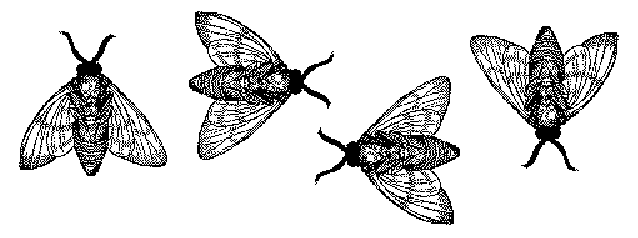
\includegraphics{flies}
\caption{A sample black and white graphic
that needs to span two columns of text.}
\end{figure*}


\begin{figure}

\includegraphics[height=1in, width=1in]{rosette}
\caption{A sample black and white graphic that has
been resized with the \texttt{includegraphics} command.}
\end{figure}

\subsection{Theorem-like Constructs}

Other common constructs that may occur in your article are the forms
for logical constructs like theorems, axioms, corollaries and proofs.
ACM uses two types of these constructs:  theorem-like and
definition-like.

Here is a theorem:
\begin{theorem}
  Let $f$ be continuous on $[a,b]$.  If $G$ is
  an antiderivative for $f$ on $[a,b]$, then
  \begin{displaymath}
    \int^b_af(t)\,dt = G(b) - G(a).
  \end{displaymath}
\end{theorem}

Here is a definition:
\begin{definition}
  If $z$ is irrational, then by $e^z$ we mean the
  unique number that has
  logarithm $z$:
  \begin{displaymath}
    \log e^z = z.
  \end{displaymath}
\end{definition}

The pre-defined theorem-like constructs are \textbf{theorem},
\textbf{conjecture}, \textbf{proposition}, \textbf{lemma} and
\textbf{corollary}.  The pre-defined de\-fi\-ni\-ti\-on-like constructs are
\textbf{example} and \textbf{definition}.  You can add your own
constructs using the \textsl{amsthm} interface~\cite{Amsthm15}.  The
styles used in the \verb|\theoremstyle| command are \textbf{acmplain}
and \textbf{acmdefinition}.

Another construct is \textbf{proof}, for example,

\begin{proof}
  Suppose on the contrary there exists a real number $L$ such that
  \begin{displaymath}
    \lim_{x\rightarrow\infty} \frac{f(x)}{g(x)} = L.
  \end{displaymath}
  Then
  \begin{displaymath}
    l=\lim_{x\rightarrow c} f(x)
    = \lim_{x\rightarrow c}
    \left[ g{x} \cdot \frac{f(x)}{g(x)} \right ]
    = \lim_{x\rightarrow c} g(x) \cdot \lim_{x\rightarrow c}
    \frac{f(x)}{g(x)} = 0\cdot L = 0,
  \end{displaymath}
  which contradicts our assumption that $l\neq 0$.
\end{proof}

\section{Conclusions}
This paragraph will end the body of this sample document.
Remember that you might still have Acknowledgments or
Appendices; brief samples of these
follow.  There is still the Bibliography to deal with; and
we will make a disclaimer about that here: with the exception
of the reference to the \LaTeX\ book, the citations in
this paper are to articles which have nothing to
do with the present subject and are used as
examples only.
%\end{document}  % This is where a 'short' article might terminate



\appendix
%Appendix A
\section{Headings in Appendices}
The rules about hierarchical headings discussed above for
the body of the article are different in the appendices.
In the \textbf{appendix} environment, the command
\textbf{section} is used to
indicate the start of each Appendix, with alphabetic order
designation (i.e., the first is A, the second B, etc.) and
a title (if you include one).  So, if you need
hierarchical structure
\textit{within} an Appendix, start with \textbf{subsection} as the
highest level. Here is an outline of the body of this
document in Appendix-appropriate form:
\subsection{Introduction}
\subsection{The Body of the Paper}
\subsubsection{Type Changes and  Special Characters}
\subsubsection{Math Equations}
\paragraph{Inline (In-text) Equations}
\paragraph{Display Equations}
\subsubsection{Citations}
\subsubsection{Tables}
\subsubsection{Figures}
\subsubsection{Theorem-like Constructs}
\subsubsection*{A Caveat for the \TeX\ Expert}
\subsection{Conclusions}
\subsection{References}
Generated by bibtex from your \texttt{.bib} file.  Run latex,
then bibtex, then latex twice (to resolve references)
to create the \texttt{.bbl} file.  Insert that \texttt{.bbl}
file into the \texttt{.tex} source file and comment out
the command \texttt{{\char'134}thebibliography}.
% This next section command marks the start of
% Appendix B, and does not continue the present hierarchy
\section{More Help for the Hardy}

Of course, reading the source code is always useful.  The file
\path{acmart.pdf} contains both the user guide and the commented
code.

\begin{acks}
  The authors would like to thank Dr. Yuhua Li for providing the
  MATLAB code of the \textit{BEPS} method.

  The authors would also like to thank the anonymous referees for
  their valuable comments and helpful suggestions. The work is
  supported by the \grantsponsor{GS501100001809}{National Natural
    Science Foundation of
    China}{http://dx.doi.org/10.13039/501100001809} under Grant
  No.:~\grantnum{GS501100001809}{61273304}
  and~\grantnum[http://www.nnsf.cn/youngscientists]{GS501100001809}{Young
    Scientists' Support Program}.

\end{acks}

\section{Introduction}

With an increased awareness of the potential for machine learning models to inadvertently amplify existing societal biases \cite{BolukbasiCZSK16a}, standards of ensuring fairness and accountability have been recently under discussion in academia, private technology companies and government institutions.  As illustrated in numerous papers including \cite{Liu2018}, the choice of model can result in drastically different impacts for subgroup populations \cite{Burke2017MultisidedFF}.  Similarly, sampling biases - either due to underlying population traits or varied subgroup population prevalence - can be grossly exaggerated in a learning classifier's output if not singularly expressed in the optimization model such as cited in \cite{Zhao2017MenAL}.
\par
Given the potential repercussions of automated tools, policy is being considered in some domains to mitigate issues of inequity. For example, in 2017 New York City introduced a bill to examine the city's *automated decision making systems* with the expressed intent of expressing transparency in algorithmic decisions \cite{NYCLaw}.  In light of these developments, the authors suggest that standards and methodologies for evaluating fairness in common edge cases scenarios are also needed as pre-requisites for potential policy decisions\cite{Adler2018, Ribeiro2016, Feldman2014}.   
\par

A common approach in fairness aware algorithms with pre-defined sensitive variables, is to set explicit sensitive variable constraints via Lagrangian relaxation enforcing a given fairness metric \cite{Menon2018TheCO}, \cite{Liu2018} etc.  However, previous work \cite{Menon2018TheCO} has established that forcing equality in the constraints is not possible unless the underlying sensitive variable subpopulations demonstrate perfect accuracy with respect to the target.  Furthermore, fairness constraints with a relaxation parameter will often result in a degradation in performance.
A separate concern is that many constraint based approaches have been implemented only in scenarios where a single sensitive variable exists and may not scale in real-world datasets where multiple subpopulations may need to be treated as *sensitive*.  In situations where multiple sensitive variables exist, there is a concern that utilizing a constrained fairness metric, such as the Equality of Odds that is referenced in this paper, will limit overall performance with an upper bound of accuracy set to the worst performing subpopulation.  
\par
Finally, hard (or soft constraints) with respect to a sensitive variable, may be inappropriate without apriori knowledge of the causal model.  In the famous Simpson's paradox found with the 1973 U.C. Berkley admissions data \cite{BerkeleyBias}, raw admissions data suggested a strong bias towards men.  However, a more thorough analysis by student major showed no discrepancy between genders. In fact the major was a confounding variable: men applied at higher rates to the easier departments in terms of acceptance. It is entirely plausible that in this scenario gender would be treated as a sensitive variable.  A global hard constraint on the sensitive variable in a classification problem would  produce noticeably different results than an algorithm optimized with the sensitive variable conditioned on major. The right approach in each scenario requires domain experts.  However, identifying potential confounding factors with respect to sensitive variables in a dataset may be an essential step in not compounding inequity \cite{Chiappa2018}. 

This paper explores the inherent trade-offs of implementing subgroup fairness via the lens of sensitive variable causality, confounding and resolving factors.  The authors posit that a metric definition of fairness using defined sensitive variables should also include:  

\begin{itemize}
\item Scaling for multiple sensitive variables
\item Addressing the influence of confounding variables via both bias exposing and resolving factors on sensitive variables
\item Metrics evaluating subgroup performance both with respect to causal relations and independent of population prevalence
\item Sample size requirements for subgroup populations 
\item Domain expert evaluation of fairness interpretation
\end{itemize}

In exploring these points we find that with an increase in the number of sensitive variables and a corresponding explosion in the dimensionality of subgroups, strict enforcement of fairness criteria may not be possible for specific joint data distributions of sensitive and non-sensitive variables. In such scenarios, we propose a softer constraint based on Pareto-efficiency \cite{Godfrey2007} which scales well with an increase in the number of subgroups. We highlight the utility of Pareto-Efficient Subgroup fairness in simple synthetic toy examples. Finally, we demonstrate that such trade-offs do exist in a real world problem consisting of the UCI Census dataset \cite{Dua:2017}.  Our proposed bias loss solution achieves Pareto-efficient performance which we argue is superior to the existing methods of equalizing loss both in terms of global and subgroup metrics. 

% \cite{Zhao2017MenAL}
% ~\cite{Menon2018TheCO}
% ~\cite{Kearns2017PreventingFG}
% ~\cite{Burke2017MultisidedFF}
% ~\cite{Beutel2017DataDA}
% ~\cite{Kleinberg2017PlanningWM}
% ~\cite{Raghavan2018TheEO}

\section{Related Work}
\subsection{Fairness Metrics}
A common mode of evaluation for fairness with respect to a sensitive variable is defined as the Equality of Odds. \cite{HardtPS16} 
\begin{definition}
\textbf{Equality of Odds} We say that a predictor $\hat{Y}$ satisfies equalized odds with respect to protected attribute $A$ and outcome $Y$, if $\hat{Y}$ and $A$ are independent conditional on $Y$.

\[  P(\hat{Y}=\hat{y}|Y=y, A=m) = P(\hat{Y}=\hat{y}|Y=y, A=n) \]
\[\forall Y, \forall m,n \in A \]

\end{definition}
This paper will explicitly utilize this metric as a standard for evaluation.

\subsection{Survey Comparison of Fairness Aware Methods}

Beutel ~\cite{Beutel2017DataDA} models the problem of debiasing as a multi-task learning problem where the model is trained to predict the output label and is  penalized if the same shared hidden layers of a feedforward neural network can be used to predict the sensitive variable accurately. The problem formulation differs from than the goals of predictive equality and avoiding disparate impact that we are seeking to achieve in our study. In their adversarial approach, the gradients are propagated such that the model is penalized when it predicts the correct sensitive variable and likewise the model is trained to predict the opposite (in case of a binary sensitive variable) of the true label. One potentially pitfall is the model could result in propagating the bias in the model, albeit in the reverse direction.

Zhao ~\cite{Zhao2017MenAL} aims to achieve corpus level parity for each of the outcomes in a classification setting. They do so by introducing Lagrangian relaxation after each iteration of the classification training. This implies that updates are approximations on each sample in the goal of achieving corpus level parity across sensitive variables. While theoretically this approach can scale to multiple bias features, the empirical behavior for the rate of convergence of the combined loss optimization of the Lagrangian approximation has not been extensively explored.

Menon and Williamson ~\cite{Menon2018TheCO} show that a disparate impact constraint is equivalent to a cost sensitive
constraint, i.e. their super-level sets are equivalent.  Similarly, they demonstrate for the mean difference (MD) score, the corresponding balanced cost sensitive risk has a cost-parameter that does not depend on $\tau$ (the MD constraint). They also formulate a fairness frontier: for a given lower bound on fairness, it measures the best excess risk over the solution without a fairness constraint. They give the theoretical limitation from which the trade-off between fairness and accuracy stems, that is dependent on the data, but not any classifier.

Kleinberg ~\cite{Kleinberg2017PlanningWM} considers two biases based on planning (present bias and sunk cost bias) and formulates the reward such that it is parameterized by (b,T) denoting the modification it makes to the final perceived reward at each step. Examples show that behaving naively or in sophisticated manner about one or both of these biases might be optimal in different conditions. The remainder of the paper isn't directly applicable to this work as it is defined as a path finding problem where rewards are adjusted by different biases and defining those parameters can be difficult.

Pleiss ~\cite{Pleiss2017} and  Raghavan ~\cite{Raghavan2018TheEO} proves that equality of odds can't be achieved by two models on separate groups which are calibrated (i.e the classification probabilities have a meaning relevant to the population), unless both the models achieve perfect accuracy. The work derives a generalized impossibility result that shows that satisfying equalized odds for more than one cost functions which capture FNR/FPR is infeasible. Empirically, they show the impact of imposing calibration and an equal cost constraint on real-world datasets. In many cases, this will result in performance degradation, while simultaneously increasing other notions of disparity.

\subsection{Potential Weaknesses with Current Fairness Metrics}

In this paper we begin to address the following possible issues with imposing fairness constraints on sensitive variables. 
% * <ananthbalashankar@gmail.com> 2018-08-21T13:46:19.689Z:
% 
% We don't address some of these in the paper, especially the first two.
% 
% ^.
\begin{enumerate}
	
	\item Impossibility Result for optimizing for Accuracy Across Sensitive Subgroups to be incompatible with Optimizing for FP and FN rates individually as shown in Figure \ref{impossibility}.
	\item Hard constraints even with relaxation factor can cause inequity across subgroups : Equality of odds cant be achieved by two models on separate groups when calibrated. 
    \item Effects of variations in prevalence and statistics across subpopulations 
    \item Confounding Factors can drastically alter interpretation of fairness across sensitive variables and without their inclusion, we may degrade performance and cause further inequity in supervised learning tasks.
\end{enumerate}

\subsection{Pareto-Efficiency}
	We seek to mitigate some of the weaknesses described above by employing Pareto-Efficiency or Pareto Optimality, an established concept in economics, engineering and life sciences.
    
\begin{definition}
\textbf{Pareto Efficiency} is a state where resources are allocated in which it is impossible to redistribute resources to make any one criterion or party better off without making another criterion worse off. 
\end{definition}

Pareto-efficiency has been extensively studied in defining trade-offs between optimizations of multiple objectives. With respect to fairness, \cite{paretoTradeoff} explores the Pareto optimality between overall accuracy and violation of fairness constraints. Although such a comparison is important and in many cases necessary by a domain expert, it is a measure of two separate metrics and needs to be carefully evaluated. In our work, we focus on the trade-offs between the performance of various subgroups which are comparable and hence the trade-offs can be easily evaluatedm simultaneously on the Pareto-optimal curve. However, in \cite{LiptonEnvyFree}, it was proved that achieving an envy free (fair) allocation of indivisible resources is a co-NP complete problem and as such we need to explore heuristic based algorithms. Study of subgroup specific performance and use of transfer learning like methods have been explored through decoupling in \cite{pmlr-v81-dwork18a}.

\begin{figure*}[htbp]
	\begin{center}
		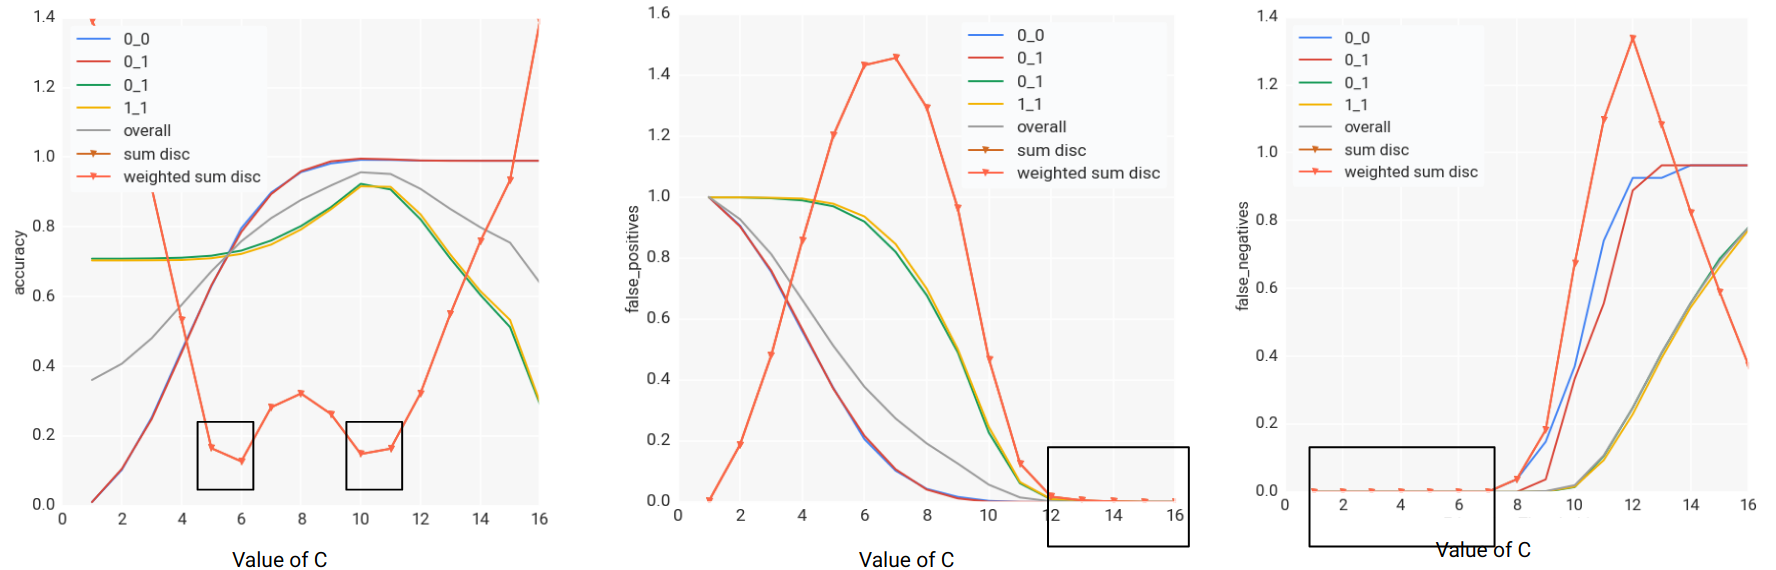
\includegraphics[width=7in,height=2.2in]{impossibility.png} 
        \setlength{\belowcaptionskip}{-8pt} 
		\caption{Example showing impossibility to equalize accuracy, FPR and FNR at the same time}
		\label{impossibility}
	\end{center}
\end{figure*}

\section{Methodology}

Given a dataset $D$ with $n$ variables, $m$ of which are considered sensitive or protected and one label in a classification task, the objective of equalized odds is to learn a model which performs equally well (be it any of accuracy, AUROC, false positive rate, true positive rate, etc) on each of the subgroups. With a complementary objective of achieving the highest overall performance, we would expect to achieve a trade-off between the two with some subgroups benefiting in performance at the cost of degradation for the others. However, in a true toy joint data distribution for two binary sensitive variables $A$ and $B$, a confounding variable $C$ and the target label $T_0$, \\
\begin{center}
Let A, B be Bernoulli random variables :
\[A \sim Bern(p)\]
\[B \sim Bern(p)\]

where $p=.5$
\begin{equation}
    Bern(p) = f(k;p) =
    \left\{
        \begin{array}{cc}
                p & \mathrm{if\ } k=1 \\
                1-p & \mathrm{if\ } k=0 \\
        \end{array} 
    \right.
\end{equation}
with a selected constant $0<c<p$
\[ C = 
\begin{cases}
\mathcal{U}(0,1) & if B = 0\\
\mathcal{N}(p, \sigma^2) - c & if B = 1, A= 0\\
\mathcal{N}(p, \sigma^2) + c & if B = 1, A= 1 \\
\end{cases}
\]

$T_0 \sim Bern(C)$ \\
\end{center}
In this scenario, there are two subgroups for which $B=0$, the confounding variable $C$ has uniform random values and for the two subgroups which have $B=1$, the confounding variable $C$ is distributed normally with means at two different values separated by a constant. Suppose we were to train a bias mitigation model $M$, which uses only the perceived non-sensitive variable "C" as the feature to classify to identify target label $T_0$  in order to achieve equal performance in terms of accuracy. While trying to increase overall accuracy, there is a potential trade-off where the algorithm could penalize two subgroups identified by $B=1$, without any gain in the subgroups identified by $B=0$. Effectively, this implies that two subgroups are penalized to ensure that accuracy is close to the uniformly random accuracy as in the other two subgroups as shown in Figure \ref{pareto}. This is counter-productive for each of the subgroup's performance in question. Hence, it is necessary to guard against such scenarios, by explicitly accounting for this edge-case.

\begin{figure}[htbp]
	\begin{center}
		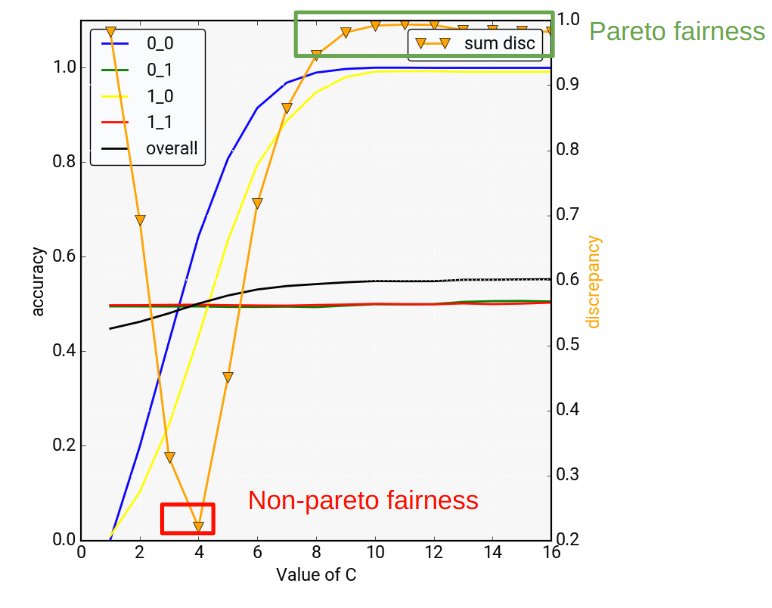
\includegraphics[width=3.2in,height=2in]{pareto.png} 
        \setlength{\belowcaptionskip}{-8pt} 
		\caption{Synthetic dataset where Pareto Efficient fairness is desirable}
		\label{pareto}
	\end{center}
\end{figure}

Our proposal is inspired from the hypothesis that the optimization should aim for "potentially optimal" performance for each of the subgroups and that "optimal" performance can be calibrated differently for different subgroups. This is similar to current research which highlights the benefits of transparency over fairness, where it is acceptable to understand the differences between various subgroups' performance in the dataset and operate in a way to correct them as opposed to fairness through blindness. Since each subgroup tries to achieve its own "optimal" performance during the course of the bias mitigation, this can be thought of achieving Pareto-efficiency, where we try to optimize for overall performance, while accepting decrease in performance for certain subgroups if and only if there is at least one subgroup which benefits as a result. We also want to ensure that the penalty is not dominated by only certain subgroups, but shared across subgroups equitably. These two constraints can be thought of as constraining the initial performance optimization objective while
minimizing the full Pareto loss $L_{p}(o, \hat{o})$. The bias mitigation objective can be specified as

\[ L_{b}(o, \hat{o}) =\min \sum{P(g)} \]
where 
\[ P(g) = Relu(F_{opt}[g] - F[g]) \]

and
$P(g \in G) < \epsilon$ for all subgroups $g$,
where G is the power set containing all possible subgroups over the set of sensitive variables $S$, $F_{opt}[g]$ is the heuristic optimal evaluation score for subgroup $g$ and $F[g]$ is the actual evaluation score for a given model and Relu is a linear activation function to avoid penalizing scores that achieve results better than the heuristic optimal one.

These constraints were relaxed through Lagrangian dual formulation similar to \cite{Eban2016} with the appropriate loss weight ($\lambda$), along with a cross entropy classification loss: $L_{ce}(o, \hat{o})$ to yield

\[ L_{p}(o, \hat{o}) = \sum(L_{ce}(o, \hat{o})) + \lambda( \sum{P(g)} + |P(g) - \epsilon| ) \]

\subsubsection{Multiple metrics of fairness}
One of the drawbacks of existing approaches, is that it isn't applied to multiple metrics of fairness like false positive rate and false negative rates simultaneously. However, the above Pareto loss can be scaled easily to mitigate discrepancy for many metrics. We achieve this by defining a penalty term per metric of fairness, weighted by separate lambdas signifying the trade-offs between the multiple Lagrangian relaxation terms. In our evaluation, we do this with an equal weighting between FPR and FNR to overcome the drawbacks of metrics like accuracy which obfuscate the type of errors in a model.

\subsection{Confounding variable detection and interpretation of fairness}
During the exploration of subgroup fairness, we were also faced with the challenge of identifying which variables were sensitive and which were not. This is usually done by the domain expert and is known ahead of time. However, due to confounding causal variables, it could be that some of the features used are highly correlated with the sensitive variable in question. It has been shown in Kilbertus et al [3] that arguing about fairness purely based on observational data is not feasible and hence the domain experts have to make decisions whether or not a particular confounding variable's bias is to be permitted. We now propose a process through which these domain experts can be aided by being presented the potential confounding variables for their decision. We present our approach based on quantifying the discrepancy in subgroup fairness in Algorithm \ref{alg:algorithm-confound} to identify potential resolving confounding variables through which we can explain the seeming bias.
 
\begin{algorithm}
\caption{Outline of Procedure for Potential Confounding Variable Detection}
\label{alg:algorithm-confound}
Given a set of sensitive features $S$, and the remaining features $F$ and a model $M$ which is  a binary classifier using the full set of features, if it turns out that the performance of $M$ on groups defined by membership in $S$ have discrepancy, we perform the following test before qualifying a model unfair.\\
For each feature $f$ in $F$, we split the population into groups based on $f$ first, and then split into subgroups based on $G$, the power set of $S$, within each of the groups.\\
We then evaluate the model $M$ on each of the subgroups and compare the performance across the subgroups.\\
For each subgroup $g \in G$, we quantify the sum of discrepancies between subgroup performance as $d[f, g]$.\\
We also quantify the lack of samples in each of the subgroups by calculating the confidence intervals of the discrepancies.\\
In some cases, some subgroups don't have enough samples to even calculate discrepancy. This is quite dangerous to ignore as we might be hiding a potentially sensitive variable whose distribution matches with one of the sensitive variables.\\
This kind of sample insufficiency will be quantified by the proportion of the population which was ignored in Step 5.\\
The confounding variable will minimize the discrepancy in Step 4, while maintaining that enough proportion of the population was used in the calculation (Step 5).\\
These are two trade-offs which can be modeled by the domain expert.\\
Return the confounding variable which can be argued as a reasoning for fairness if the discrepancy calculated in Step 4 is close to zero.\\
\end{algorithm}

We will argue the other case (where it seems fair, but could be interpreted given further information as not) similarly. Only, in that case, we aim to identify variables which maximize discrepancy instead of minimizing. Since these variables expose subgroup bias when conditioned on them, these can also be considered potentially sensitive if the domain expert determines that the bias from such confounding variables are to be mitigated. We present the next few sections assuming that the set of sensitive variables are already updated with some of these confounding variables included as determined by the domain expert.

\subsection{Pareto-Efficent Algorithm}
In order to obtain a heuristic of the optimal subgroup performance, we use the performance achieved when trained purely on the subgroup's data in question. We understand that this isn't the best estimate in many cases, especially where prevalence of subgroups are varied, and majority subgroups benefit from a large dataset, whereas minority subgroups can be penalized as we avoid any transfer learning \cite{PapernotAEGT16}. We hence propose an iterative approach where this heuristic would be updated in each iteration if the optimal subgroup performance was bettered by a jointly trained model. In the rest of the evaluation, we present results from the heuristic initialized with the separately trained performance for better understanding of our approach. Once we obtain the heuristic optimal performances, we input them into the jointly training Pareto bias mitigation algorithm, which minimizes the loss $L_p$ mentioned above for every batch. We further ensure that the batch used at every loss minimization is representative of the subgroup distribution present in the original dataset.

\begin{algorithm}
\caption{Iterative Pareto-Efficient Bias Mitigation}
\label{alg:algorithm-pareto}
\begin{algorithmic}
\STATE{G = $\mathcal{P}(S)$ where S is the membership set of sensitive variables}
\STATE{$F_{opt}(g) = eval(M_{g}, D_{g})$  $\forall g \in G$, $M_{g}$ is the model trained and evaluated on only $D_{g}$, data with subgroup g}
\STATE{$F = \{\}$}
\WHILE{F is $\{\}$ or $\exists g, F[g] > F_{opt}[g]$}
\STATE{Update $F_{opt}[g] = F[g]$ if $F[g] > F_{opt}[g]$}
\STATE{Train M to minimize $L_p$ for the updated $F_{opt}$}
\STATE{$F[g] = eval(M, D_{g})$}
\ENDWHILE
\end{algorithmic}
\end{algorithm}

\subsection{Bias Loss Weights}
The loss to be minimized contains a single bias loss weight term which we use to control the trade off between overall accuracy and achieving Pareto-efficient levels for each of the subgroups with equal penalty per subgroup. This term influences the decisions and changing this weight further exemplifies the difference between the equalized odds loss and the Pareto loss as can be seen in Figure \ref{bias_weight}. As we increase the bias weight, we see that the Pareto loss bias mitigation moves to other Pareto-efficient levels with higher overall accuracy, whereas the equalized loss moves towards the undesired operating point where discrepancy across subgroups is minimized regardless of improvement in accuracy by at least one of the subgroups. We can also weigh the discrepancies of each of the subgroups differently, but our synthetic datasets did not warrant it. We leave it to the practitioner to correspondingly set these weights per subgroup or as a constant as needed. 

\begin{figure*}[htbp]
	\begin{center}
		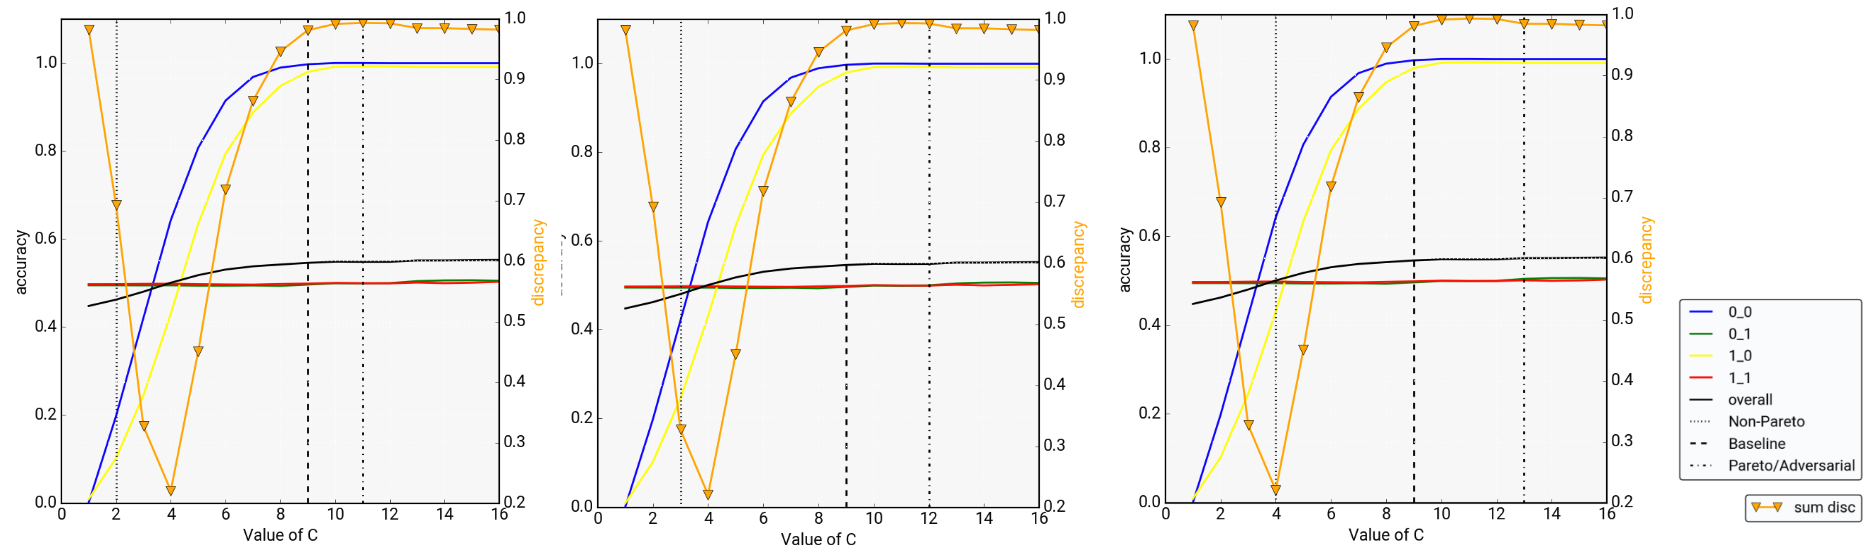
\includegraphics[width=7.5in,height=2.4in]{bias_weight.png} 
        \setlength{\belowcaptionskip}{-8pt} 
		\caption{Effect of bias weight on bias trade-offs}
		\label{bias_weight}
	\end{center}
\end{figure*}

\subsection{Prevalence}
Prevalence usually varies between subgroups and some minority subgroups could be ignored during bias mitigation. The appproach mentioned in Kearns et al. \cite{Kearns2017PreventingFG} defines discrepancies factoring the population ratio of each of the subgroups. This can have perverse effects on these subgroups as their performance deviating from either the overall performance or the Pareto-efficient level can be ignored while optimizing the loss function. This is clearly seen in Figure \ref{prevalence} where the discrepancy curve representing the discrepancy from the overall performance can be seen to have lowered and smoothened when multiplied with the subgroup's population ratio. This can be quite deceiving where the majority subgroup, which also guides the overall performance dominates the sum of discrepancy loss too. Hence, we guard against such prevalence based weighting.

\begin{figure}[htbp]
	\begin{center}
		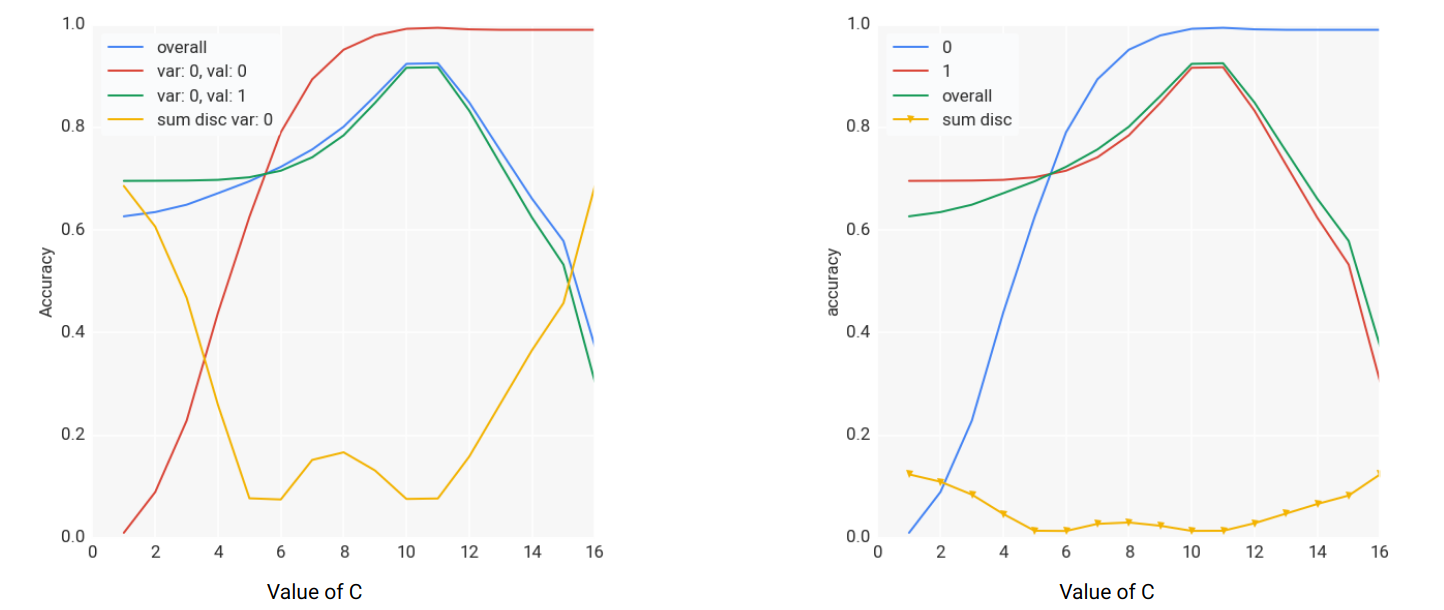
\includegraphics[width=3.2in,height=2.0in]{prevalence.png} 
        \setlength{\belowcaptionskip}{-8pt} 
		\caption{Weighing discrepancy by prevalence ignores the minority subgroup}
		\label{prevalence}
	\end{center}
\end{figure}




 
 



\section{Evaluation}

We compare our approach with the scaled versions of group fairness \cite{Zhao2017MenAL} and \cite{Beutel2017DataDA} for subgroups. In \cite{Zhao2017MenAL}, Zhao, et al. optimize for overall accuracy in the constrained setting of ensuring equal false positive rates, but is generally applicable to other measures of performance. For our comparison we implement a Lagrangian relaxation which adds penalty for each subgroup that deviates from the overall accuracy. In \cite{Beutel2017DataDA}, Beutel et al, they implement bias mitigation as a way of forgetting the sensitive group membership by back-propagating negative gradients in a multi headed feedforward neural network. We scale the same for subgroups defined over multiple sensitive variables, where the auxiliary head aims to predict the subgroup class (multi-class classification instead of binary).

\subsection{Synthetic Data}
We perform the comparison for both synthetic toy data with the setup similar to the use case mentioned in the above section and the UCI Census Adult dataset where based on demographic information, the task is to predict the income category. The sensitive variables considered in this task are gender and race.

Table \ref{tab:synthetic_subgroups} shows that for many of the synthetic cases where it is possible for all subgroups to achieve same level of accuracy, we see that our approach remains similar in subgroup performance \cite{Zhao2017MenAL} and \cite{Beutel2017DataDA}. However, for the use case where some subgroups differ in their "optimal" performance, \cite{Zhao2017MenAL} fails to achieve the "optimal" accuracy for all subgroups and hence results in lower overall accuracy. \cite{Beutel2017DataDA} however continues to perform equally well, similar to our approach in these scenarios.

\begin{table}[tp]
\footnotesize

\caption{UCI Adult dataset with bias mitigation algorithms}
\begin{center}
\begin{tabular}{lccccc}
\hline
\textbf{Model} & \textbf{Accuracy} & \textbf{FPR} & \textbf{FNR} & \textbf{Discrepancy} & \textbf{Pareto Loss}\\\hline
Baseline (no bias loss) & 0.630 & 0.253 & 0.747 & 0.199 & 0.016\\
Minimize Discrepancy & 0.619 & 0.283 & \textbf{0.712} & \textbf{0.167} & 0.133\\
Adversarial Loss & 0.648 & 0.224 & 0.769 & 0.226 & 0.077\\
Pareto-Efficient Loss & \textbf{0.678} & \textbf{0.165} & 0.830 & 0.250 & \textbf{0.000}\\\hline
\end{tabular}
\end{center}
\label{tab:uci_comparison}
\normalsize
\end{table}%

\begin{table}[tp]
\footnotesize
\caption{Change in overall accuracy as compared to baseline on synthetic dataset}
\begin{center}
\begin{tabular}{lccc}
\hline
\textbf{\vtop{\hbox{Confounding dependency}\hbox{Mean of normal distribution}}} & \textbf{Pareto} & \textbf{Minimize Discrepancy} & \textbf{Adversarial}\\\hline
2*a + 1*b & 0 & 0 & 0\\
2*b - 2*a & 0 & 0.02 & 0.02\\
4*b & 0 & 0 & -0.002\\
8*b & 0 & -0.06 & 0\\
2*a + 2*b + 2*d & 0 & 0 & 0\\
\vtop{\hbox{\strut (a,b): \{(0,0): 3, (0,1): 11,}\hbox{\strut (1,0): 4, (1,1): 8\}}}
 & 0 & 0 & 0\\
\vtop{\hbox{\strut (a,b): \{(0,0): 3, (0,1): 1,}\hbox{\strut (1,0): 4, (1,1): 8\}}}
 & 0 & -0.04 & -0.04\\
\vtop{\hbox{\strut (a,b): \{(0,0): 3, (0,1): 11,}\hbox{\strut (1,0): 4, (1,1): 9\}}}
 & 0 & -0.01 & -0.01\\
\vtop{\hbox{\strut (a,b): \{(0,0): 3, (0,1): 11,}\hbox{\strut (1,0): 4, (1,1): 9\}}\hbox{Prevalence ratio: 1:9:1:9}}
 & 0 & \textbf{-0.1} & 0\\\hline
\end{tabular}
\end{center}
\label{tab:synthetic_subgroups}
\normalsize
\end{table}%

\subsection{UCI Census Data}
Table \ref{tab:uci_comparison} shows that for the UCI Census Adult dataset, \cite{Zhao2017MenAL} performs significantly well in terms of lowering the discrepancy of the subgroup's accuracy from the overall accuracy (measured in discrepancy). This is expected as per the objective that \cite{Zhao2017MenAL} set out to achieve. \cite{Beutel2017DataDA} achieves similar, but comparatively worse and our approach performs the worst as compared to the baseline which did not have any bias mitigation. However, the scenario is different when considering the Pareto Loss, i.e the penalty that each subgroup deviates from the optimal of the respective subgroup. We see that our approach achieves zero Pareto-Loss, while \cite{Zhao2017MenAL} and \cite{Beutel2017DataDA} have significant Pareto losses. Table \ref{tab:uci_subgroups} clarifies why this is the case, where we see that each of the subgroups have better accuracy, some even better than the baseline than all the other approaches. This again, is evident from the objective function which we set out to achieve, where each group is trying to achieve their heuristic optimal performance (quoted in the last row of Table \ref{tab:uci_subgroups}).

\begin{table}[tp]
\footnotesize
\caption{Subgroup performance on UCI Adult dataset}
\begin{center}
\begin{tabular}{lccccc}
\hline
\textbf{Model} & \textbf{Subgroup 1} & \textbf{2} & \textbf{3} & \textbf{4} & \textbf{Pareto Loss}\\\hline
Baseline (no bias loss) & 0.890 & 0.883 & 0.818 & 0.784 & 0.016\\
Minimize Discrepancy & 0.853 & 0.856 & 0.806 & 0.778 & 0.133\\
Adversarial Loss & 0.882 & 0.872 & 0.824 & 0.780 & 0.077\\
Pareto-Efficient Loss & \textbf{0.935} & \textbf{0.915} & \textbf{0.844} & \textbf{0.797} & \textbf{0.000}\\
Subgroup Pareto Frontier & 0.934 & 0.894 & 0.815 & 0.783 & N/A \\\hline
\end{tabular}
\end{center}
\label{tab:uci_subgroups}
\normalsize
\end{table}%

\subsection{Effect of Model capacity}
We used 3 layers of feed forward networks with 256, 128 and 64 neurons fully connected in all our comparisons of relevant losses. However, we did notice that the difference in the losses varied with the size of the model used as noted in Table \ref{tab:uci_model_size}. The gains achieved from Pareto loss is higher when the model capacity increases, as it is able to capture the per subgroup specific performance updates with more number of parameters.

\begin{table}[tp]
\footnotesize
\caption{Effect of model size on subgroup performance (compared with baseline) on UCI Adult dataset}
\begin{center}
\begin{tabular}{lcccc}
\hline
\textbf{Model size} & \textbf{Subgroup 1} & \textbf{2} & \textbf{3} & \textbf{4}\\\hline
64 & 0.923 (0.929) & 0.898 (0.914) & 0.812 (0.849) & 0.733 (0.809)\\
$128,64$ & 0.902 (0.925) & 0.884 (0.909) & 0.820 (0.849) & 0.781 (0.805)\\
$256,128,64$ & \textbf{0.935} (0.890) & \textbf{0.915} (0.883) & \textbf{0.844} (0.818) & \textbf{0.797} (0.784)\\\hline
\end{tabular}
\end{center}
\label{tab:uci_model_size}
\normalsize
\end{table}%


\subsection{Confounding Variable Detection}
To detect the potential confounding variables in the UCI Census dataset, we first ran the baseline logistic regression model to predict income bracket, without the sensitive variables: race and gender. We then evaluated the performance of each of the subgroups when conditioned on values of each of the other feature variables to calculate the subgroup discrepancy for each variable. If the subgroup discrepancy conditioned on a feature is less than a upper threshold,  $\alpha$, then we might define those features as potential resolving variables. So potentially, within a bound of discrepancy  $\alpha$, we can explain away all the subgroups discrepancy by conditioning on such features. Similarly, if the subgroup discrepancy when conditioned on a features is more than a lower threshold $\beta$, such variables are defined as unresolving variables and expose the discrepancy within the subgroups. For continuous variables such as education, we quantize the values into 10 levels and plot their discrepancy as shown in Figure \ref{edu_disc}. Potential confounding variables can also be easily compared quantitatively using the lower and upper thresholds for subgroup discrepancy as shown in Figure \ref{all_disc}.

\begin{figure}[htbp]
	\begin{center}
		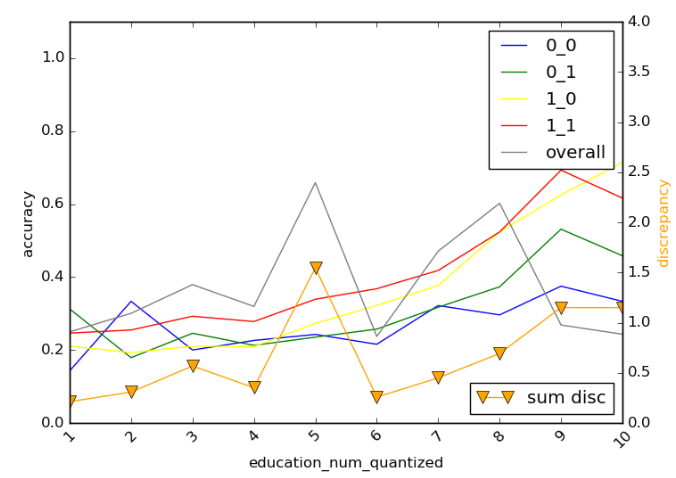
\includegraphics[width=3.2in,height=1.6in]{education_disc.png} 
        \setlength{\belowcaptionskip}{-8pt} 
		\caption{Education as a potential confounding variable in the UCI Census dataset($\alpha=1.6, \beta=0.2$)}
		\label{edu_disc}
	\end{center}
\end{figure}

\begin{figure*}[htbp]
\centering  
\subfigure[Hours per week ($\alpha=1.1, \beta=0.1$)]{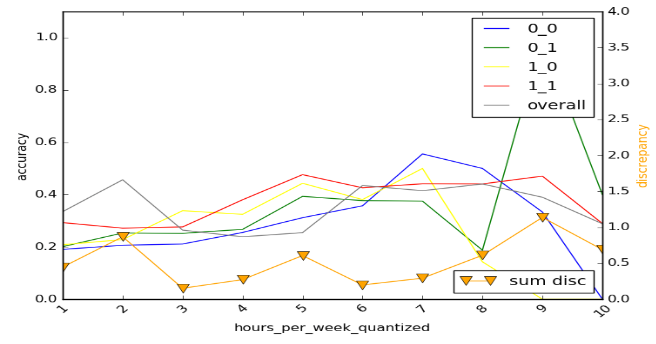
\includegraphics[width=0.45\linewidth]{age_disc}}
\subfigure[Occupation ($\alpha=2.0, \beta=0.05$)]{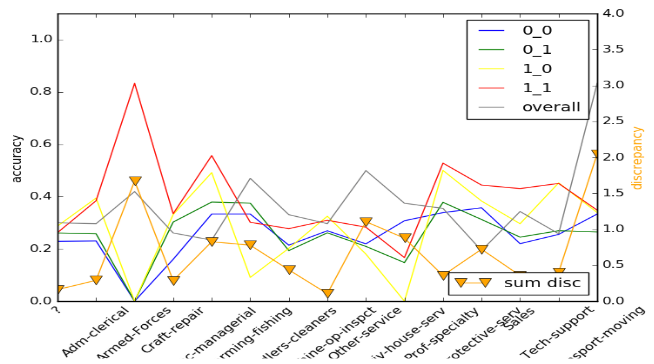
\includegraphics[width=0.45\linewidth]{occupation_disc}}
\subfigure[Relationship ($\alpha=0.9, \beta=0.1$)]{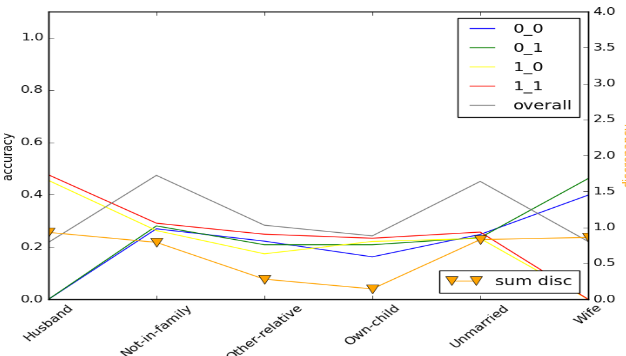
\includegraphics[width=0.45\linewidth]{relation_disc}}
\subfigure[Age ($\alpha=1.5, \beta=0.01$)]{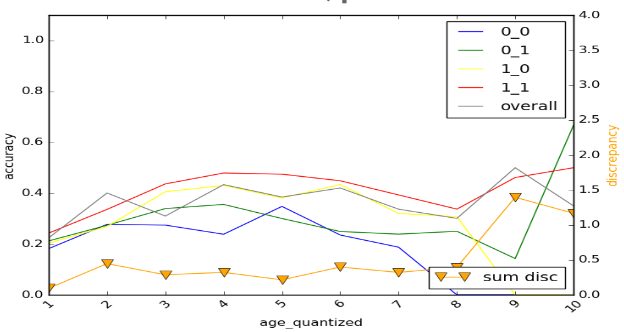
\includegraphics[width=0.45\linewidth]{age_q_disc}}
\caption{Potential confounding variables in UCI Census dataset with their corresponding thresholds of discrepancy}
\label{all_disc}
\end{figure*}



\subsection{Summary of Results}
	In this paper we sought to establish several points, in the application of sensitive variable constraints in the spirit of fairness for  machine learning models. 
\begin{enumerate}
	\item \textbf{Influence of Confounding Factors} - In order to perform a macro analysis of the trade-offs in fairness, possible confounding factors in relation to sensitive variables need to identified.  Without apriori knowledge of causality, a statistical analysis can only hypothesis variable effect.  In this paper, we suggest a standard for identifying possible confounding variables in relation to pre-defined sensitive variables. Similarly, we suggest incorporating the possible confounding variables into the sensitive variable subgroup constraints to mitigate their effects.  \par
    	In essence this approach is examining the individual conditional posterior probabilities for each subgroup.  The authors acknowledge that this approach will grow exponentially with the number of sensitive variables and possible confounding variables. As such this solution is only appropriate for a limited number of sensitive variables within a dataset. \par
    
    \item \textbf{Evaluate Subgroups Individually} - When more than one sensitive variable is present, evaluating subgroups individually and predicated on possible confounding factors mitigates the effects of prevalence on a dataset.  In real world problems, the population of subgroups with combinations of sensitive variables is unlikely to be equivalent and often skewed to a dominant sub-population. Similarly when sample populations are heavily skewed in prevalence, metrics such as accuracy can be deceptive and entirely mis-categorize a minority subgroup. In enforcing sensitive variable constraints, the authors are motivated to apply such Lagrangian constraints to individually to BOTH the False Positive and False Negative Loss functions for each subgroup.  
    
    \item \textbf{Dynamic Subgroup Fairness Constraints}  - The paper attempted to identify several instances where fixed accuracy constraints for individual subpopulations, even with a relaxation parameters, would be inappropriate for real-world datasets. In fact, fixed constraints may perform sub-optimally increasing inequity. The paper offers a Pareo-Efficient algorithm and methodology to address this scenario. As dissected in Menon et. al \cite{Menon2018TheCO}, there will be a degradation in performance due to a fairness constraint unless the existing subgroup populations have equivalent possible sample accuracies. The algorithm in this paper, using an optimal heuristic derived either from experiments with the existing data or another method such as transfer learning, mitigates the cited global(macro) and subgroup(micro) performance degradation.  As demonstrated in Table \ref{tab:uci_subgroups}, the accuracy for each subgroup  in the UCI dataset is noticeably improved with the paper's Pareto-Efficient Loss methodology. Similarly the global accuracy is improved. 
 \end{enumerate}
   
 
 
 
 
 
    

    

\section{Conclusion}
	In this paper we have established an algorithm and methodology to address confounding factors in a dataset as well as to mitigate performance degradation and further inequity when establishing subgroup constraints in a machine learning problem.  The solution proposed in this paper utilizing softer tailored subgroup optimization performance constraints is appropriate for problems with multiple  fixed sensitive variables that demonstrate differing sampling population statistics in terms of prevalence, accuracy etc.  As demonstrated in the toy dataset experiments, the proposed methodology will not degrade performance in terms of accuracy for datasets that do not demonstrate the edge-cases described. In fact, we demonstrated a substantial increase in global accuracy and individual subgroup accuracy as compared to existing proposed fairness algorithms. \par
    
However, we note two potential concerns with the approach:
\begin{itemize}
	\item \textbf{Scaling Sensitive Variables and Confounding Factors}  The algorithm requires a thorough analysis of individual subgroup population combinations or apriori knowledge.  This will increase exponential with the number of assigned sensitive variables and/or possibly identified confounding variables.  Similarly, multiple variables will greatly increase the initial pre-processing and evaluation time.
 	\item \textbf{Subgroup Sample Size} The paper's approach is predicated on examining the individual subgroup populations. As the number of variables grow, the sample size  required for these population in order to establish optimal statistics may not be possible. For example, it is within reason, to consider a scenario where a subgroup can be reduced to a possible sample size of 1. This scenario is not addressed in this paper, but is of considerable importance when exploring sensitive variable constraints in ML as applied in policy decisions.  
\end{itemize}

In future work, we hope to explore subgroup sample population bounds as a possible aid in establishing fairness requirements at a policy level.

%\pagebreak


















% Bibliography 
\bibliographystyle{ACM-Reference-Format}
\bibliography{sample-bibliography}

\end{document}
